\section{}
\textbf{NOTE: } the values of $t_I=3$ has been used as $t_I=2$ leads to the infection dying out in around 20 days.
The three strategies used where as follows:

\textbf{Global:} In this strategy, we select nodes with largest degree from the Susceptible set, then vaccinate them.

\textbf{Local:} This strategy focused on the fringe of the infection.
Here a subset of susceptible is created, where every node with a infected or vac. \& infected neighbour is included in this subset.
Then nodes with the highest number of neighbours who are infected or vac. \& infected are selected to be vaccinated.
This approximately selects nodes with the highest probability of being infected in the next simulation step.

\textbf{Local - 2 Step:} This strategy is an expansion of the \textbf{local} strategy. 
Here we still calculate the number of infected neighbours of every node on the infected fringe, approximating the risk of infection.
But now we introduce another lookahead step that looks at how many susceptible neighbours each node on the fringe has, approximating the risk of infecting others.
Multiplying the risk of infection and risk of infecting others gives us a danger level of each node in the fringe.
We then select fringe nodes with the highest danger level to vaccinate.  

\begin{figure}[h!]
    \begin{center}
        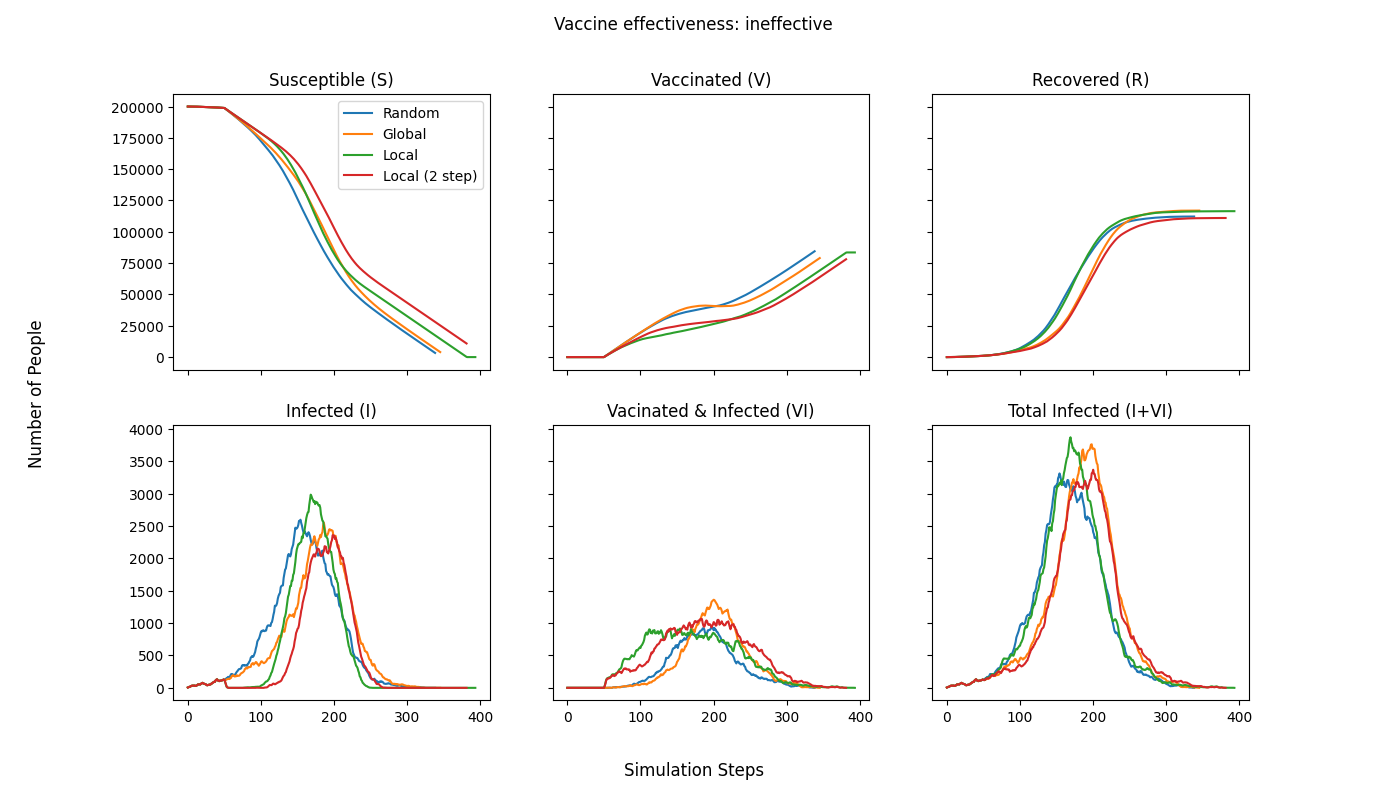
\includegraphics[width=1\textwidth]{Q6-none.png}
        \caption{Figure showing the how changing the vaccination strategy effects the course of an outbreak. Red - random strategy. Yellow - globally target nodes of highest degree. Green - target nodes of highest degree on infection fringe. Local (2 step) - an extension of the local strategy that targets nodes most at risk 2 steps in the future.} 
        \label{fig:q6-none}
    \end{center}
\end{figure}


\begin{figure}[h!]
    \begin{center}
        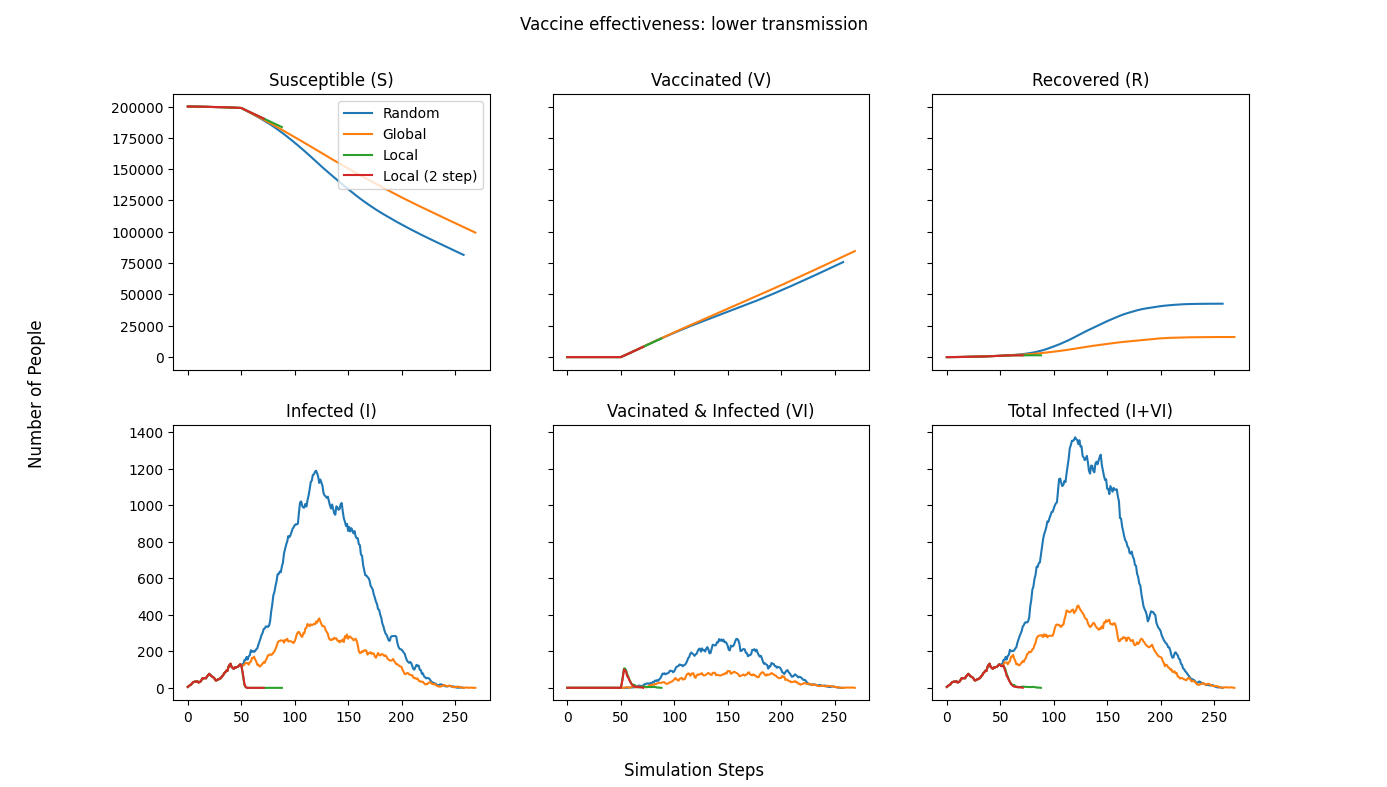
\includegraphics[width=1\textwidth]{Q6-transmit.png}
        \caption{Figure showing the how changing the vaccination strategy effects the course of an outbreak. Red - random strategy. Yellow - globally target nodes of highest degree. Green - target nodes of highest degree on infection fringe. Local (2 step) - an extension of the local strategy that targets nodes most at risk 2 steps in the future.} 
        \label{fig:q6-transmit}
    \end{center}
\end{figure}


\begin{figure}[h!]
    \begin{center}
        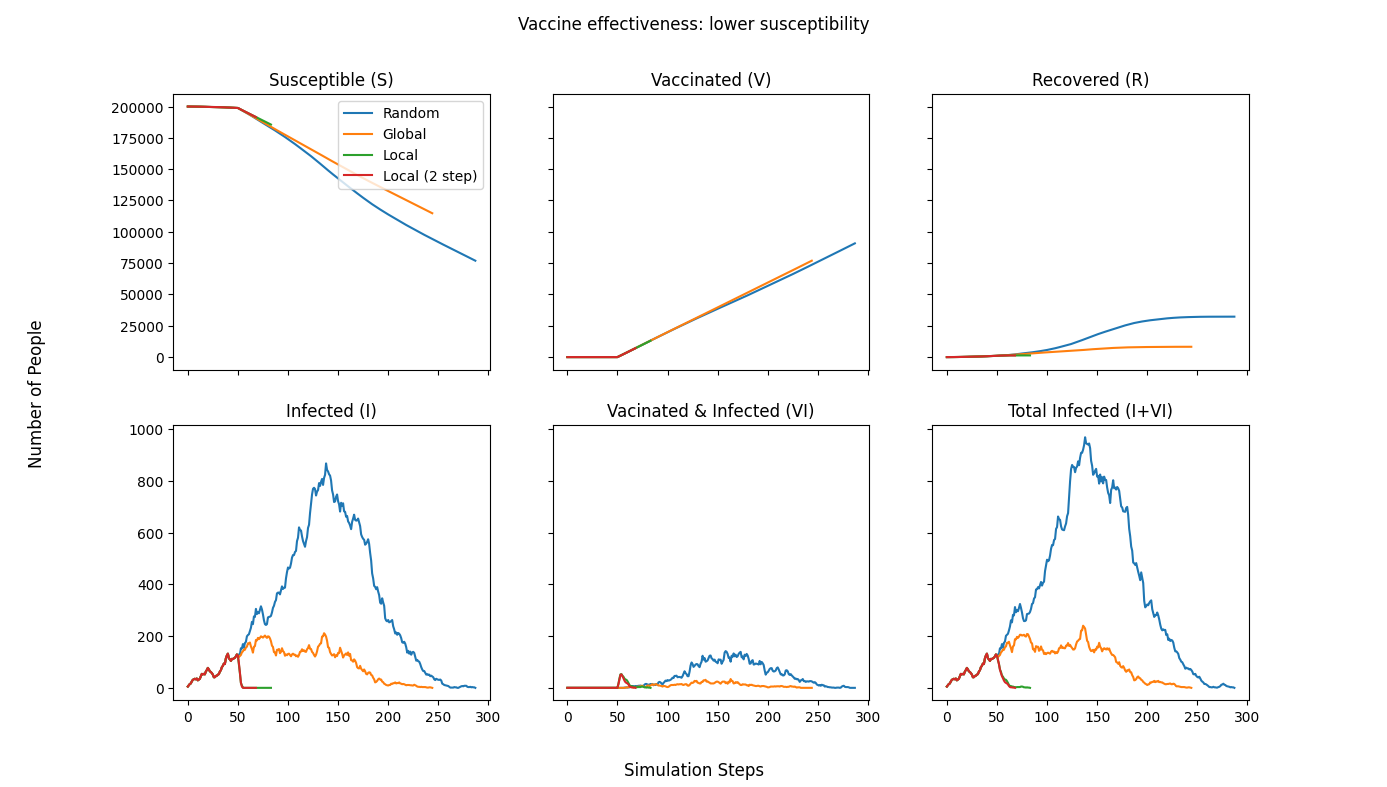
\includegraphics[width=1\textwidth]{Q6-catch.png}
        \caption{Figure showing the how changing the vaccination strategy effects the course of an outbreak. Red - random strategy. Yellow - globally target nodes of highest degree. Green - target nodes of highest degree on infection fringe. Local (2 step) - an extension of the local strategy that targets nodes most at risk 2 steps in the future.} 
        \label{fig:q6-catch}
    \end{center}
\end{figure}


\begin{figure}[h!]
    \begin{center}
        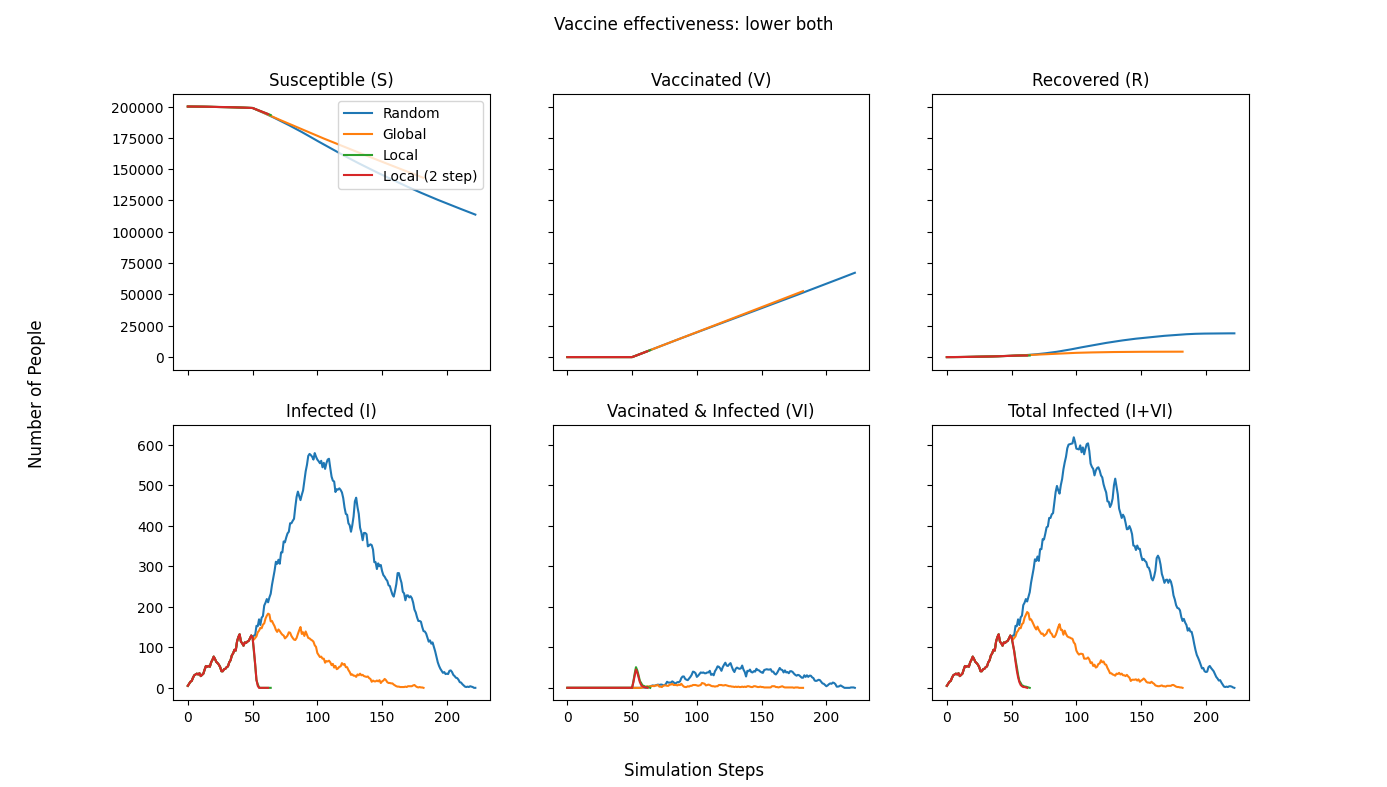
\includegraphics[width=1\textwidth]{Q6-both.png}
        \caption{Figure showing the how changing the vaccination strategy effects the course of an outbreak. Red - random strategy. Yellow - globally target nodes of highest degree. Green - target nodes of highest degree on infection fringe. Local (2 step) - an extension of the local strategy that targets nodes most at risk 2 steps in the future.} 
        \label{fig:q6-both}
    \end{center}
\end{figure}


Looking at Figure \ref{fig:q6-transmit}, \ref{fig:q6-catch},\ref{fig:q6-both} we can see that all 3 strategies out preform the random vaccination strategy.
The \textbf{global} strategy consistently reduces the total number of infections, while mildly shortening the length of the outbreak.
The \textbf{local} and \textbf{local - 2 step} strategies are very effective at containing outbreak.
For every effective vaccine we observe that at day 50 onwards there is a step drop of infections, with thee outbreak ending before 100 days.
The \textbf{2 step} has a very similar performance to the \textbf{local} strategy, although it is mildly more effective at eliminating the infection with marginally shorter outbreak periods.   